\documentclass{article}
\usepackage{xcolor}
\usepackage{titleps}
\usepackage[letterpaper, margin=0.95in]{geometry}
\usepackage{url}
\usepackage{amsmath}
\usepackage{amssymb}
\usepackage{wrapfig}
\usepackage{float}
\usepackage{mathtools}
\usepackage{enumitem}
\usepackage{tabu}
\usepackage{parskip}
\usepackage{natbib}
\usepackage{listings}
\usepackage[utf8]{inputenc} % allow utf-8 input
\usepackage[T1]{fontenc}    % use 8-bit T1 fonts
\usepackage[hidelinks]{hyperref}       % hyperlinks
\usepackage{wrapfig}
\usepackage{url}            % simple URL typesetting
\usepackage{booktabs}       % professional-quality tables
\usepackage{amsfonts}       % blackboard math symbols
\usepackage{nicefrac}       % compact symbols for 1/2, etc.
\usepackage{microtype}      % microtypography
\usepackage{xcolor}         % colors
\usepackage{amsmath,amssymb} % define this before the line numbering.
\usepackage{makecell}
% % Support for easy cross-referencing
\usepackage{graphicx} % for pdf, bitmapped graphics files
\usepackage{subcaption}
\usepackage{colortbl}
\usepackage{xcolor}
% \usepackage{epsfig} % for postscript graphics files
\usepackage{empheq}
%\usepackage{mathptmx} % assumes new font selection scheme installed
% \usepackage{times} % assumes new font selection scheme installed
\usepackage{bm}
\usepackage{bbding}
% \usepackage{cite}
\usepackage{diagbox}
\usepackage[linesnumbered,ruled]{algorithm2e}
% \usepackage{ulem} %to strike the words
% \usepackage{hyperref}
% \usepackage{soul}

\newcommand{\cmark}{\ding{51}}%
\newcommand{\xmark}{\ding{55}}%
% \definecolor{themeblue}{RGB}{57, 162, 219}
% \definecolor{themegreen}{RGB}{87, 204, 153}
% \definecolor{forestgreen}{RGB}{47, 159, 87}

\usepackage[capitalize]{cleveref}
% \usepackage{todonotes}
\usepackage{float}
\usepackage{booktabs}
\usepackage{multirow}
%\usepackage{ bbold }
\usepackage{mathrsfs}
\usepackage[utf8]{inputenc}
%\usepackage{subfigure}
\usepackage{pifont}
\usepackage{threeparttable}

\usepackage{hyperref}
\usepackage[color=red]{todonotes}
\usepackage{forest}
\definecolor{light-yellow}{HTML}{FFE5CC}
\newcounter{RNum}
\renewcommand{\theRNum}{\arabic{RNum}}
\newcommand{\Remark}{\noindent\textbf{Remark}~\refstepcounter{RNum}\textbf{\theRNum}: }
\newcommand{\fref}[1]{Fig.~\ref{#1}}
\newcommand{\sref}[1]{Section~\ref{#1}}
\newcommand{\tref}[1]{Table~\ref{#1}}
\newcommand{\appref}[1]{Appendix~\ref{#1}}
\newcommand{\highlight}[1]{\noindent\quad\textbf{#1}:~}
\newcommand{\myparagraph}[1]{\noindent\textbf{#1}~}

\newpagestyle{ruled}
{\sethead{CMU 16-831}{Intro to Robot Learning}{Fall 2024}\headrule
  \setfoot{}{}{}}
\pagestyle{ruled}

\renewcommand\makeheadrule{\color{black}\rule[-.75\baselineskip]{\linewidth}{0.4pt}}
\renewcommand*\footnoterule{}

\begin{document}
\lstset{basicstyle = \ttfamily,columns=fullflexible,
  backgroundcolor = \color{light-yellow}
}

\begin{centering}
  {\Large Assignment 1: Imitation Learning} \\
  \vspace{.25cm}
  \textbf{Andrew ID:} \texttt{mukaiy} \\
  % \textbf{Collaborators:} \texttt{YOUR COLLABORATORS}\\
\end{centering}

\vspace{.5cm}

\section{Behavioral Cloning (65 pt)}
\subsection{Part 2 (10 pt)}
\begin{table}[!h]
  \centering
  \begin{tabular}{cccccc}
    \toprule[1.0pt]
    Metric/Env & Ant-v2          & Humanoid-v2     & Walker2d-v2    & Hopper-v2        & HalfCheetah-v2  \\
    \midrule
    Mean       & 4713.6533203125 & 10344.517578125 & 5566.845703125 & 3772.67041015625 & 4205.7783203125 \\
    Std.       & 12.196533203125 & 20.9814453125   & 9.237548828125 & 1.9483642578125  & 83.038818359375 \\
    \bottomrule[1.0pt]
  \end{tabular}%
  \label{tab:p2}%
\end{table}%

\subsection{Part 3 (35 pt)}
\begin{table}[htbp]
  \centering
  \begin{tabular}{ccccc}
    \toprule[1.0pt]
    Env    & \multicolumn{2}{c}{Ant-v2} & \multicolumn{2}{c}{Humanoid-v2}                                                \\
    \midrule
    Metric & Mean                       & Std.                            & Mean                     & Std.              \\
    Expert & 4713.6533203125            & 12.196533203125                 & 10344.517578125          & 20.9814453125     \\
    BC     & 4714.01708984375           & 93.93411254882812               & 248.40753173828125 (???) & 55.91537094116211 \\
    \bottomrule[1.0pt]
  \end{tabular}%
  \label{tab:p3}%
  \caption{Run with \textit{--eval\_batch\_size 5000 --num\_agent\_train\_steps\_per\_iter 10000}}
\end{table}%

\subsection{Part 4 (20 pt)}

\begin{figure*}[!ht]
  \centering
  \begin{subfigure}[b]{.49\linewidth}
    \centering
    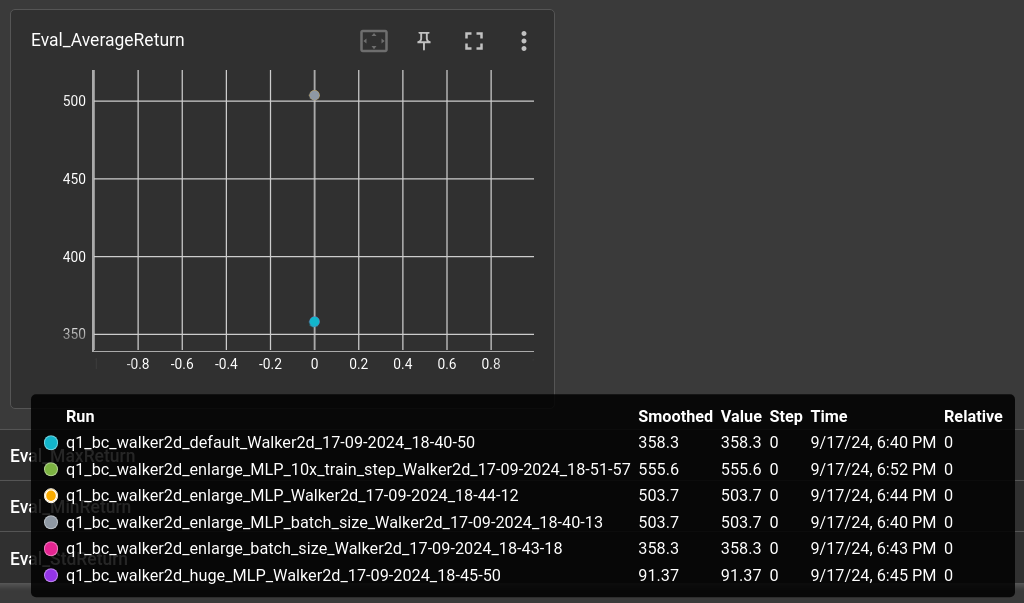
\includegraphics[width=\columnwidth]{figs/bc_walker2d_average_return.png}
    \caption{Average Return.}
  \end{subfigure}
  \begin{subfigure}[b]{.49\linewidth}
    \centering
    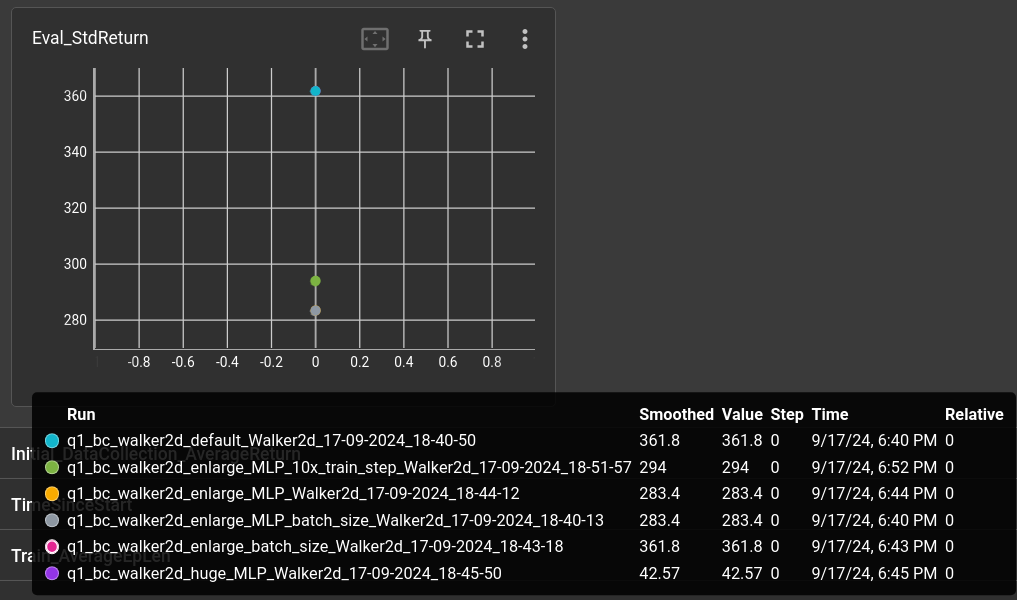
\includegraphics[width=\columnwidth]{figs/bc_walker2d_standard_return.png}
    \caption{Std Return.}
  \end{subfigure}
  \caption{BC agent's performance varies with the value of batch size, training step, MLP size parameters in Walker 2D environment.}
  \label{fig:p4}
\end{figure*}

Experiment with Humanoid failed because of the complexity of observation (state) space (376 vs Ant's 111), could not improve with noticeable margin.
Walker 2D has far less DoF (17 vs Ant's 111), but the dynamics is non-trivial.

All the experiment are conducted with \textit{--eval\_batch\_size 5000}, detailed setup and results are in \tref{tab:p4}.

\begin{table}[!h]
  \centering
  \begin{tabular}{c|cccccc}
    \toprule[1.0pt]
    Setup          & Default & enlarge\_batch\_size & enlarge\_MLP & huge\_MLP        \\
    \midrule
    Batch size     & 1000    & 10000                & 1000         & 1000             \\
    Training step  & 1000    & 1000                 & 1000         & 1000             \\
    MLP depth      & 2       & 2                    & 5            & 10               \\
    MLP size       & 64      & 64                   & 128          & 256 (512 failed) \\
    \midrule
    Average Return & 358.3   & 358.3                & 503.7        & 91.37            \\
    Std Return     & 361.8   & 283.4                & 283.4        & \textbf{42.57}   \\
    \bottomrule[1.0pt]
  \end{tabular}
  \begin{tabular}{c|cccccc}
    \toprule[1.0pt]
    Setup          & enlarge\_MLP\_batch\_size & enlarge\_MLP\_10x\_train\_step \\
    \midrule
    Batch size     & 10000                     & 1000                           \\
    Training step  & 1000                      & 10000                          \\
    MLP depth      & 5                         & 5                              \\
    MLP size       & 128                       & 128                            \\
    \midrule
    Average Return & 503.7                     & \textbf{555.6}                 \\
    Std Return     & 283.4                     & 294                            \\
    \bottomrule[1.0pt]
  \end{tabular}
  \caption{Experiment Setup.}
  \label{tab:p4}
\end{table}

\textbf{Analysis:}

The dominant factor is the MLP depth/size and training step, increasing batch size does not help much. The huge MLP failed because of the overfitting issue, and the huge MLP size 512 failed because of the exploding/vanishing gradient issue.

\section{DAgger (35 pt)}
\subsection{Part 2 (35 pt)}
\begin{figure*}[h!]
  \centering
  \begin{subfigure}[b]{.99\linewidth}
    \centering
    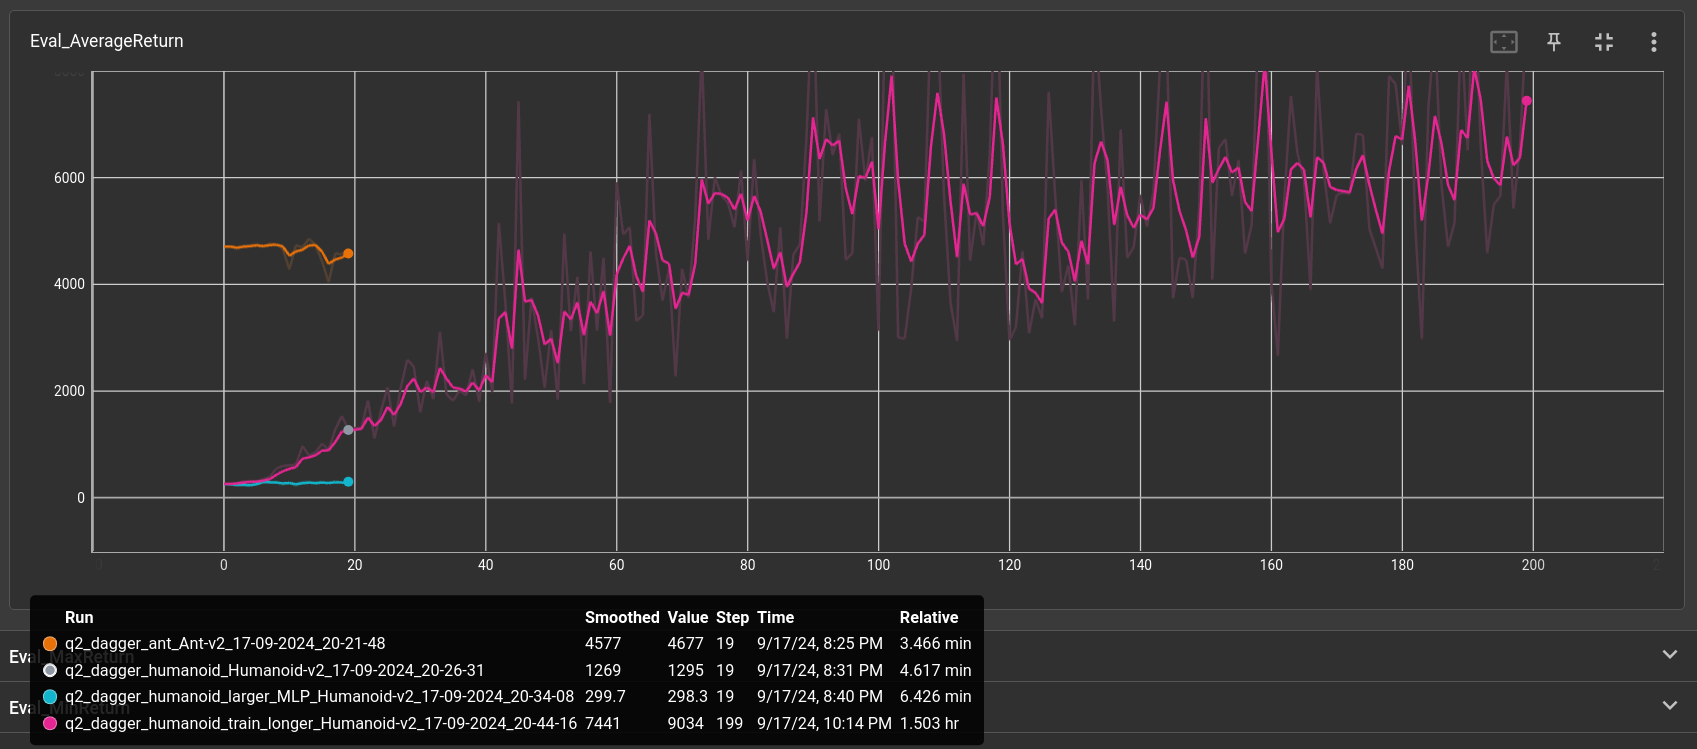
\includegraphics[width=\columnwidth]{figs/DAgger_average_return.png}
    \caption{Average Return.}
  \end{subfigure}
  \begin{subfigure}[b]{.99\linewidth}
    \centering
    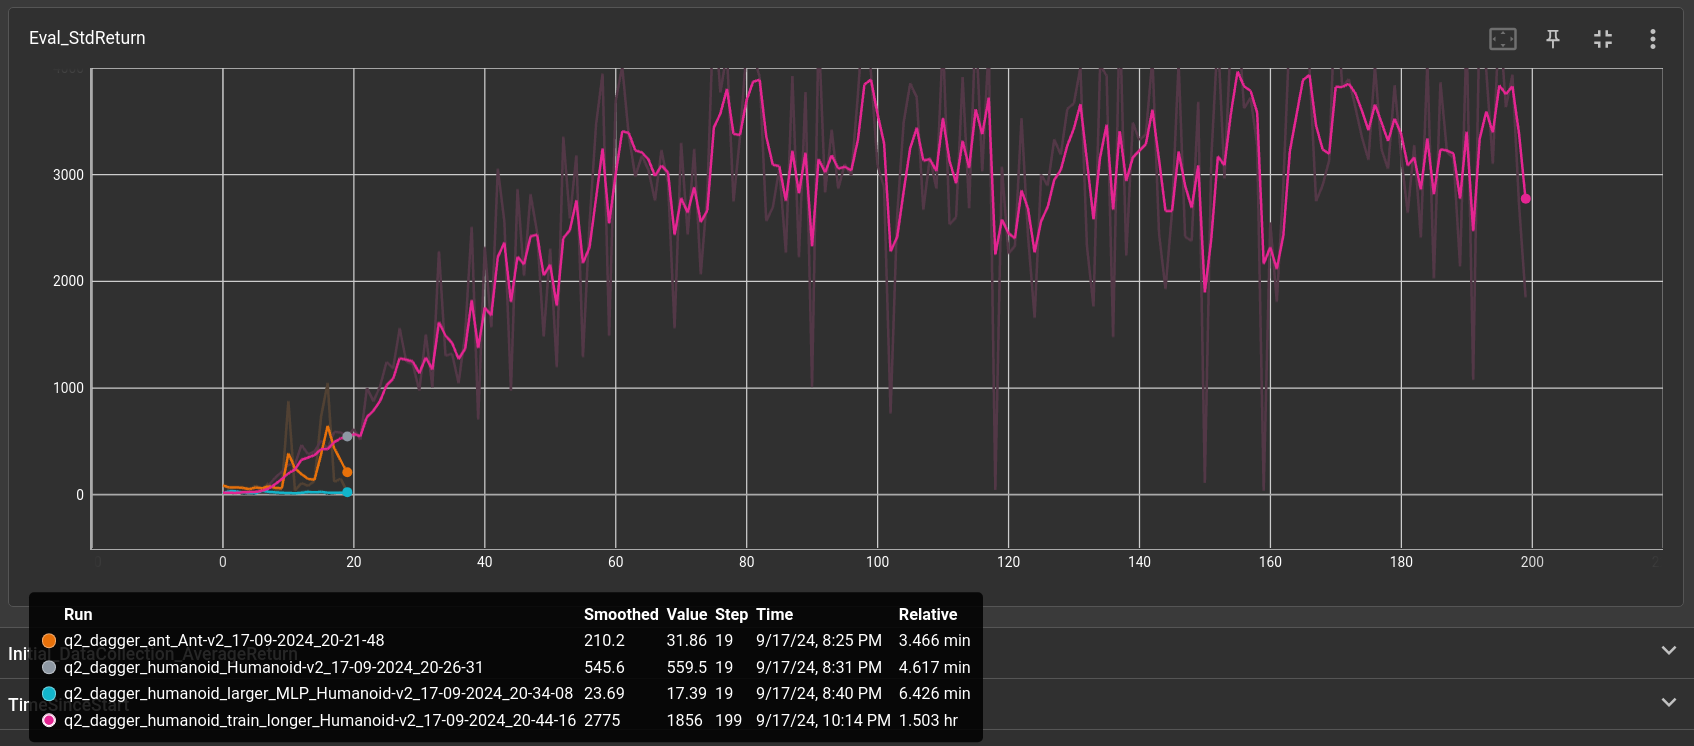
\includegraphics[width=\columnwidth]{figs/DAgger_std_return.png}
    \caption{Std Return.}
  \end{subfigure}
  \caption{Learning curve of DAgger agent in Ant-v2 and Humanoid-v2 environment.}
  \label{fig:p5}
\end{figure*}

\begin{figure*}[h!]
  \centering
  \begin{subfigure}[b]{.49\linewidth}
    \centering
    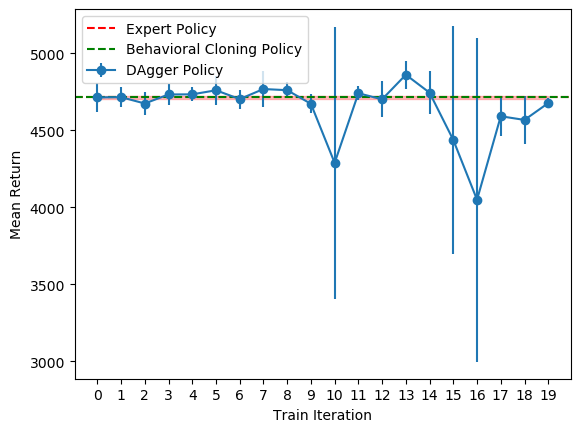
\includegraphics[width=\columnwidth]{figs/ant_DAgger.png}
    \caption{Ant-v2.}
  \end{subfigure}
  \begin{subfigure}[b]{.49\linewidth}
    \centering
    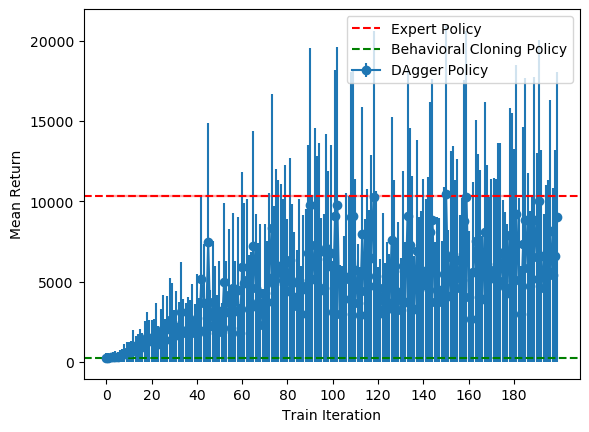
\includegraphics[width=\columnwidth]{figs/humanoid_DAgger.png}
    \caption{Humanoid-v2.}
  \end{subfigure}
  \caption{Mean Return vs Train Iteration with error bar and expert performance.}
  \label{fig:p6}
\end{figure*}

Result is shown in \fref{fig:p5} and \fref{fig:p6}.

\textbf{Analysis:}

Ant agent in \textcolor{orange}{orange curve} is already doing a good job in non-DAgger Behavioral Cloning.

In comparison, Humanoid agent's performance gets improved a lot by DAgger as expected.
Increasing the depth and size of MLP does not help much compared to the default setting, so the Humanoid agent is trained with the default setting for the 200-iteration run in \textcolor{magenta}{magenta}.

Training DAgger agent with iterations more than 100 does not improve much, possibly due to the network architecture.

The standard deviation of the return is high in the Humanoid environment, which is expected because of the complexity of the environment.
The Humanoid expert agent with such a low std at 20.98 must have been trained with a more sophisticated architecture/method.

\end{document}
